\subsubsection{الگوی \lr{Safety Executive}}
\label{archSafeSafetyExecSec}
\begin{RTL}
این الگو \cite{ref4}
برای سیستم‌هایی طراحی شده است که اقدامات ایمنی پیچیده‌ای دارند
و نمی‌توان آنها را به سادگی با خاموش کردن سیستم به دست آورد.
این الگو یک جزء مجری ایمنی معرفی می‌کند تا چندین کانال
و اقدامات ایمنی را مدیریت و هماهنگ کند و سیستم را از طریق
یک سری مراحل به وضعیت ایمن هدایت کند. این الگو به‌ویژه برای سیستم‌هایی
که با مواد خطرناک یا حالت‌های پرانرژی کار می‌کنند و خاموشی فوری می‌تواند
خطرناک باشد، مفید است. پیاده‌سازی این الگو پیچیده است و معمولاً
برای سیستم‌های بسیار حساس به ایمنی استفاده می‌شود و در
چنین محیط‌هایی حفاظت عالی در برابر خطا ارائه می‌دهد.
\end{RTL}
\begin{figure}[h!]
\centering
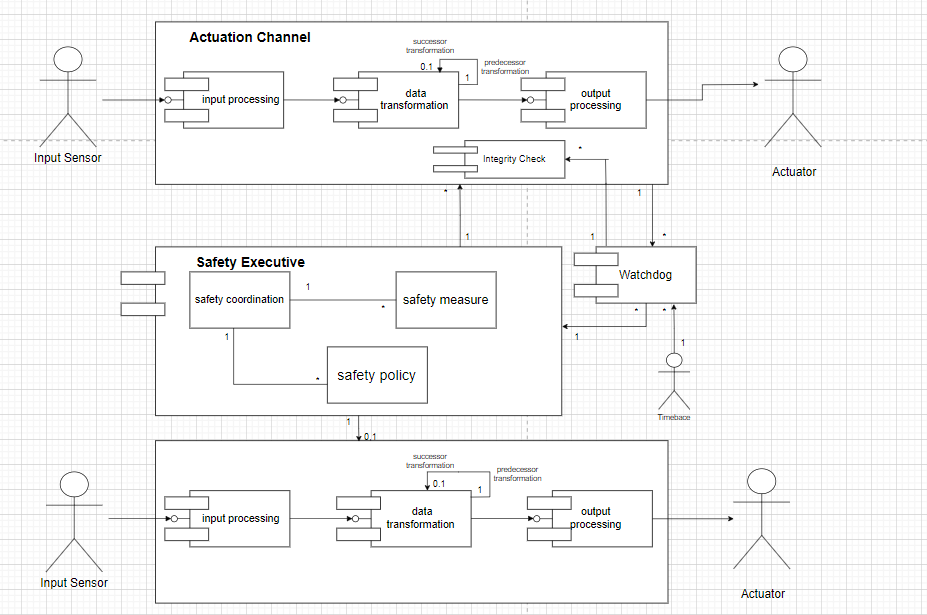
\includegraphics[scale=0.5]{images/third/safetyExec.png}
\caption{ساختار الگوی \lr{Safety Executive}}
\end{figure}